\section{Introduzione}
\textcolor{blue}{\lipsum[1-2]}
\section{Background}

L'identificazione di sistemi è un insieme di tecniche che si prefigge lo scopo di identificare i parametri e il sistema tale da descrivere un certo fenomeno. La prima grande distinzione vede la separazione di due tecniche: identificazione parametrica e non parametrica. La prima parte stimando un modello del fenomeno e punta ad identificare i parametri che lo rappresentano. L'identificazione non parametrica, invece, procede senza conoscere il modello del fenomeno, al più ne stima alcune caratteristiche, e punta ad identificare il sistema che meglio lo descrive.

In questo caso si parte da un modello ben noto, un modello di meccanica polmonare lineare descritto da un circuito RLC, e se ne identificano i parametri descrittivi.

\subsection{Sistema RLC}

Il circuito RLC (\cref{fig:RLC}) permette, seguendo l'analogia elettrica, di descrivere un modello approssimato della meccanica respiratoria. Il modello prevedere una serie di resistenza, induttore e capacità. Sulla base dell'analogia tra la corrente elettrica e il flusso polmonare è possibile rappresentare, in un modello a parametri concentrati, le componenti di compliance e resistenza elastica dei polmoni \cite{ghafarian_review_nodate}. 

Questo modello permette di affrontare i casi fisiologici in cui il flusso entrante nei polmoni è predominante rispetto al flusso bloccato (flusso che invece aumenta notevolmente in caso di patologie ostruttive). L'analogia vede l'associazione della differenza di pressione alla differenza di potenziale, la corrente al flusso d'aria e l'induttanza come un'inertanza, ovvero la differenza di pressione richiesta per causare una variazione unitaria nel tasso di variazione del flusso nel tempo. 

In un caso paziente specifico sarebbero necessarie misure sperimentali così da ottenere il modello reale sul quale effettuare l'identificazione. In questo caso, non avendo a disposizione dati sperimentali, si utilizzano dei dati noti in letteratura \cite{khoo_physiological_2018}. 

\begin{itemize}
	\item $\operatorname{R}=0.1  \:\left[\text{cmH2O s}\over \text{L} \right]$
	\item $\operatorname{L}=0.01 \:\left[\text{cmH2O s}^2\over \text{L} \right]$
	\item $\operatorname{C}=0.1 \:\left[\text{L}\over \text{cmH2O} \right]$
\end{itemize}

In questo modello semplificato si considerano un'unica resistenza e un'unica compliance che vanno a rappresentare la complessiva e la capacità di accumulare aria del sistema respiratorio nel suo complesso. Quindi la resisitenza $\operatorname{R}$ porta con se il contributo resistivo delle vie aeree, dei tessuti polmonari e della parete toracica. La capacità $\operatorname{C}$ rappresenta il compliance dei tessuti e della parete toracica.

L'obiettivo è la predizione della pressione alveolare $p_A$ e della sua risposta dinamica a differenti forme d'onda di pressione applicare all'apertura delle vie aeree $p_{ao}$.

Applicando la prima legge di Kirchoff al circuito in \cref{fig:RLC} si ottiene:

\begin{equation}
p_{a O}=L \frac{d i}{d t}+R i+p_{a}
\end{equation}

Dove vale il legame:

\begin{equation}
	i=C \frac{d p_{a}}{d t}
\end{equation}

Da cui si ricava la funzione di trasferimento:

\begin{equation}
	H(s)=\frac{P_{a}(s)}{P_{ao}(s)}=\frac{1}{1+s R C+s^{2} L C}
\end{equation}

Questo mostra come $p_a$ è interamente dipendente da $p_{ao}$ e il sistema è un sistema con configurazione open-loop. 

\begin{figure}[b!]
	\centering
	\small{
	\def\svgwidth{0.8\linewidth}
	\input{lung_model.pdf_tex}}
	\caption{Astrazione di polmoni, parete toracica e spazio pleurico}
	\label{fig:model}
\end{figure}

\begin{figure*}[t]
	\begin{subfigure}{0.5\linewidth}
		\centering
		 	\small{\def\svgwidth{0.85\linewidth}
	\input{RLC.pdf_tex}}
	\caption{}
	\end{subfigure}\hfill
	\begin{subfigure}{0.5\linewidth}
		\centering
	\def\svgwidth{0.8\linewidth}
	\input{RLC_tf.pdf_tex}
	\caption{}
\end{subfigure}
\caption{Circuito RLC rappresentante la meccanica polmonare (a); sistema open loop rappresentante il circuito RLC (b)}
\label{fig:RLC}
\end{figure*}

\subsection{Identificazione dei parametri}

Non avendo a disposizione dati paziente specifici sulla meccanica respiratoria i dati verranno generati tramite la procedura \texttt{rlc\_fun.m} che restituisce la risposta del circuito RLC fornendogli in ingressi i parametri del sistema. 

A questo può essere aggiunto anche del rumore.

\subsection{Algoritmo di Nelder–Mead}

Una volta assunto come modello del sistema la funzione di trasferimento di un circuito RLC, per stimare i parametri è necessario definire una funzione obiettivo. Tale funzione rappresenta la differenza tra la risposta misurata (vera) del sistema e quella stimata:

\begin{equation}
\underline e=\underline y^{\operatorname{pred}} - \underline y^{\operatorname{mis}}
\end{equation}

E la ricerca dei parametri corretti punta alla minimizzazione della funzione obiettivo definita come:

\begin{equation}
 \mathrm{E}={1\over 2} \|\underline e\|^2
 \label{eq:obj}
\end{equation}

Uno dei possibili modi per affrontare questo problema consiste nell'affidarsi alla routine di \texttt{Matlab} nota come \texttt{fminsearch()}. Tale procedura si occupa di restituire i parametri ottimali. In particolare, questa funzione sfrutta l'algoritmo di Nelder Mead \cite{lagarias_convergence_1998}. Tale metodo non fa uso di derivate e si basa sul concetto di un simplesso approssimando il punto di ottimo locale in $n$ variabili. 


\subsection{Metodo di Gauss-Newton}

Un'alternativa è il metodo di Gauss-Newton. Il metodo, diversamente dal precedente, richiede di portare in conto anche le derivate. 

La minimizzazione dell'\cref{eq:obj} è un problema non lineare ai minimi quadrati. La soluzione numerica sfrutta il metodo di Gauss Newton. Come il metodo di Newton, si impone la stazionarietà, condizione che si riflette sulla j\textsuperscript{ma} compnente:

\begin{equation}
	(\nabla \mathrm {E})_{j}=\sum_{k} e_{k} \cdot \frac{\partial e_{k}}{\partial p_{j}}
\end{equation}

Ovvero tale differenziazione corrisponde a premoltiplicare per la matrice di sensibilità J:
\begin{equation}
\nabla \mathrm{E}=\underline{\underline{J}}^{T} \underline{e}
\end{equation}

Utilizzando quindi l'algoritmo di Newton l'iterazione al passo $k+1$ cercherà i parametri ($\underline p$) come:
\begin{equation}
\underline{p}^{(k+1)}=\underline{p}^{(k)}-\left.[\nabla \left(\nabla \mathrm E\right)]^{-1} \left(\nabla \mathrm E \right)\right|_{\underline{p}^{k}}	
\end{equation}

Per l'approssimazione introdotta da Gauss \cite{nocedal_numerical_2006} è possibile trascurare le componenti quadratiche dovute alla derivata seconda: 

\begin{equation}
	\begin{aligned}
	(\nabla^2 \mathrm{E})_{i j}=\frac{\partial \mathrm{E}}{\partial p_{j} \partial p_{j}}&=\frac{\partial}{\partial p_{i}}\left(e_{k} \frac{\partial e_{k}}{\partial p_{j}}\right)\\&=\frac{\partial e_{k}}{\partial p_{i}} \frac{\partial e_{k}}{\partial p_{j}}+\cancel{e_{k} \frac{\partial^{2} e_{k}}{\partial p_{j} \partial p_{i}}}	
	\end{aligned}	
\end{equation}

Ovvero considerare l'iterazione semplicemente come:

\begin{equation}
\underline{p}^{(k+1)}=\underline{p}^{(k)}+\underline h^{(k)}
\end{equation}

Dove l'incremento sarà:

\begin{equation}
\underline h^{(k)}=-\left.\left[\underline{\underline{J^{T}}} \:\underline{\underline{J}}\right]^{-1} \cdot \underline{\underline{J}}^{T} \underline{\underline{e}}\right|_{\underline{p}}(k)
\end{equation}

\section{Metodi}

Dunque il problema di identificazione parametrica viene affrontato come un problema di minimizzazione che porta a trovare i parametri ottimali. Sono quindi riportate le due differenti analisi.


\subsection{Minimizzazione}

Nel primo metodo si utilizza la routine di \texttt{Matlab} \texttt{fminsearch()}. La risposta vera del sistema viene calcolata tramite la routine \texttt{rlc\_fun.m} che si occupa, una volta fornitegli i coefficienti $R,\:L,\:C$ e l'ingresso, la risposta del sistema dinamica. Una volta generati i dati corrispondenti alla risposta vera del sistema è possibile procedere all'ottimizzazione. 

Si richiama allora la procedura \texttt{fminsearch()} fornendogli la funzione obiettivo, il punto iniziale e le variabile necessarie per il calcolo della funzione obiettivo (ingresso e discretizzazione temporale). La funzione obiettivo è presente all'interno della routine \texttt{onj\_fun.m} e si occupa di fare la differenza tra l'uscita vera e quella predetta. L'uscita predetta viene calcolata ad ogni iterazione sfruttando la procedura di \texttt{rlc\_fun.m} andando a calcolare la risposta del sistema RLC con i parametri aggiornati di volta in volta mediante l'algoritmo di Nelder-Mead. 

Effettuando un primo test, con rumore gaussiano, è possibile stimare i parametri. 

Inoltre, è possibile estrarre alcune informazioni dal processo di ottimizzazione. In particolare, si vede come nonostante la risposta del sistema viene stimata correttamente (\cref{fig:primo_test_4_parametri}), l'errore sui parametri è piuttosto alto (\cref{tab:test_3_param}).

\begin{table}
\begin{tabular}{|c|c|c|c|c|}
	\hline
	& Vero & Iniziale & Stimato & Errore relativo \\
	\hline
	$R$ & 0.100 & 0.150 & 0.119 & 0.197 \\
	\hline
	$L$ &  0.010 & 0.008 & 0.012 & 0.206 \\
	\hline
	$C$ & 0.100 & 0.280 & 0.083 & 0.169 \\
	\hline
\end{tabular}
\caption{Risultati dell'ottimizzazione con \texttt{fminsearch()} considerando 3 parametri.}
\label{tab:test_3_param}
\end{table}

\begin{figure}
	\centering
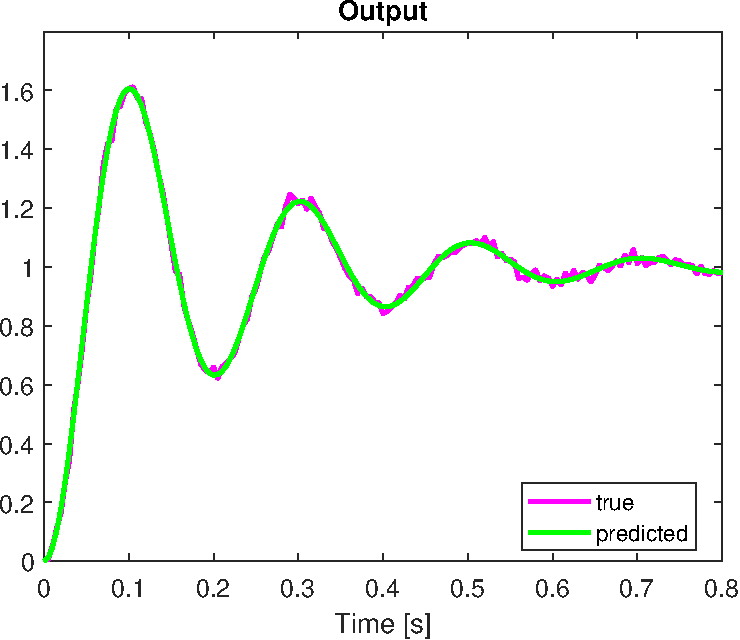
\includegraphics[width=\linewidth]{primo_test_4_parametri}
\caption{Confronto tra la risposta vera (con aggiunta di rumore gaussiano) e la risposta stimata dopo aver ottimizzato i parametri (caso iniziale con 3 parametri). La risposta viene stimata correttamente e la procedura di stima va ad effettuare una sorta di filtraggio del rumore.}
\label{fig:primo_test_4_parametri}
\end{figure}

\subsection{Non identificabilità strutturale}

Il problema, per come è stato posto, presenta una formulazione sbagliata. Infatti, andando a calcolare la matrice di sensibilità si vedono alcuni problemi. La matrice di sensibilità non è altro che l'insieme delle derivate della misura n\textsuperscript{ma} rispetto al j\textsubscript{mo} parametro. Calcolando quindi numericamente lo Jacobiano è possibile fare alcune considerazioni. 
Per calcolarlo è sufficiente perturbare rispetto al j\textsuperscript{mo} parametro e calcolarne la derivata come rapporto incrementale tra la risposta del sistema con ingresso perturbato e lo stato non perturbato rispetto la perturbazione:
\begin{equation}
	J_{i}={y_{\operatorname{pert}}-y_{\operatorname{ref}}\over |\operatorname{pert_i}|}
\end{equation}

I risultati numerici mostrano come la matrice ha un numero di condizionamento molto alto $1.856 \:10^7$ ma sembrerebbe avere rango massimo. Tuttavia, andando ad indagare i valori singolari si vede come uno dei tre è in realtà molto piccolo, abbastanza da poter essere considerato numericamente nullo. Nonostante il software percepisce un numero diverso da zero questo è in realtà nullo ed indica come nel problema c'è una dipendenza tra i parametri.

Questo è legato al fatto che nella risposta di trasferimento in realtà i parametri sono soltanto due, dati dal prodotto dei tre valori numerici legati ai componenti circuitali:
\begin{equation}
	\begin{aligned}
		\theta_1&=L*C\\
		\theta_2&=R*C
	\end{aligned}
\end{equation}

\subsection{Parametri ottimi}

Considerando quindi il problema nella sua versione ben condizionata è possibile procedere a stimare i parametri $\theta_1$ e $\theta_2$. 
In particolare è possibile analizzare il risultato ottenuto considerando diversi ingressi, mostrati in \cref{fig:inputs}.

\begin{figure*}
\begin{subfigure}{0.25\linewidth}
	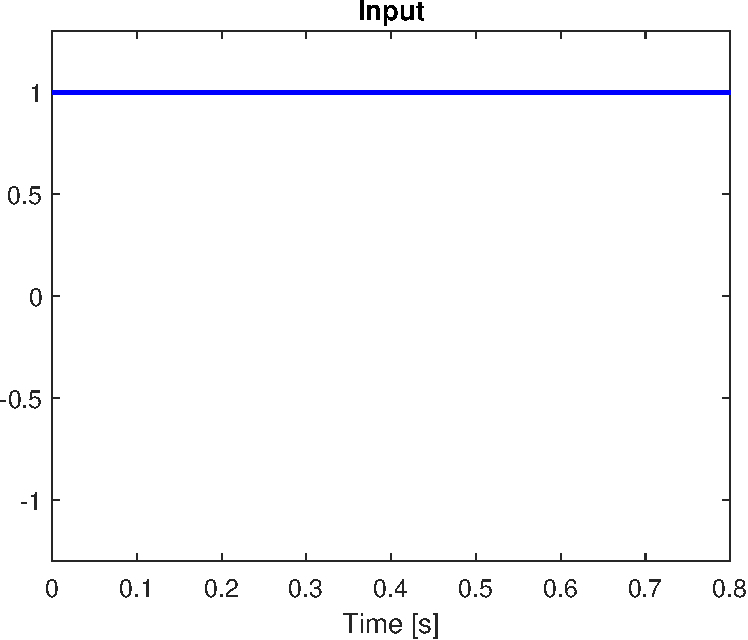
\includegraphics[width=0.9\linewidth]{step}
	\caption{}
\end{subfigure}\hfill
	\begin{subfigure}{0.25\linewidth}
	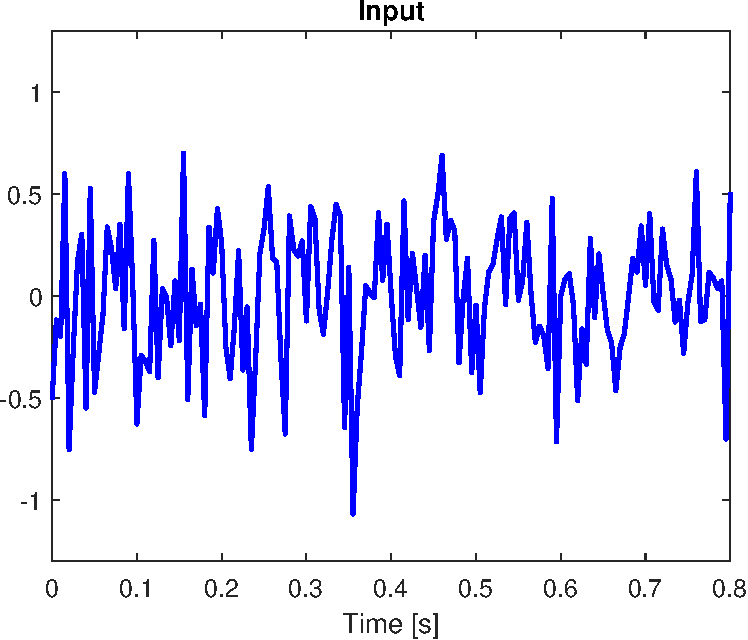
\includegraphics[width=0.9\linewidth]{rgs}
	\caption{}
\end{subfigure}\hfill
	\begin{subfigure}{0.25\linewidth}
	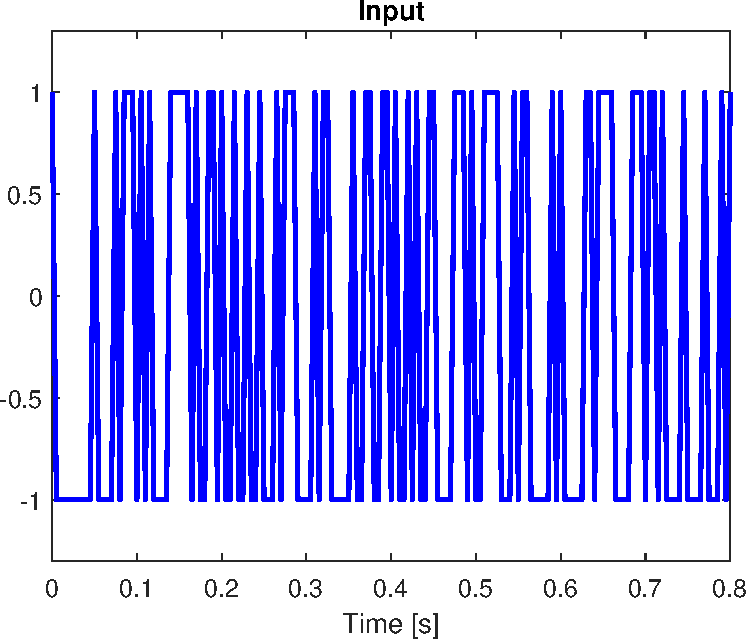
\includegraphics[width=0.9\linewidth]{rbs}
	\caption{}
\end{subfigure}\hfill
	\begin{subfigure}{0.25\linewidth}
	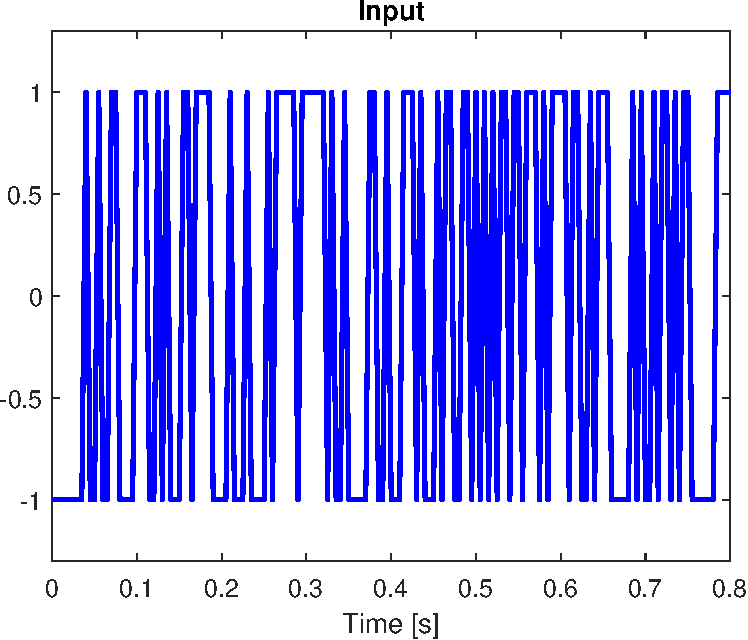
\includegraphics[width=0.9\linewidth]{prbs}
	\caption{}
\end{subfigure}\hfill
	\caption{Differenti ingressi utilizzati per stimolare il sistema RLC. Ingresso a gradino (a); ingresso di tipo binario random (b); segnale gaussiano random (c); segnale binario pseudorandomico (d). I segnali sono stati generati tramite il comando \texttt{idinput()} appositamente per l'identificazione di sistemi \cite{idinput}.}
	\label{fig:inputs}
\end{figure*}

Per farlo viene riorganizzato il codice in modo da racchiudere la generazione dei dati e l'ottimizzazione in due procedure che possono essere richiamate di volta in volta con i differenti ingressi. Con tutti gli ingressi testati l'errore rimane sotto il 2\% pur mantenendo una certa variabilità tra le differenti iterazioni. 

\begin{figure}
	\centering
	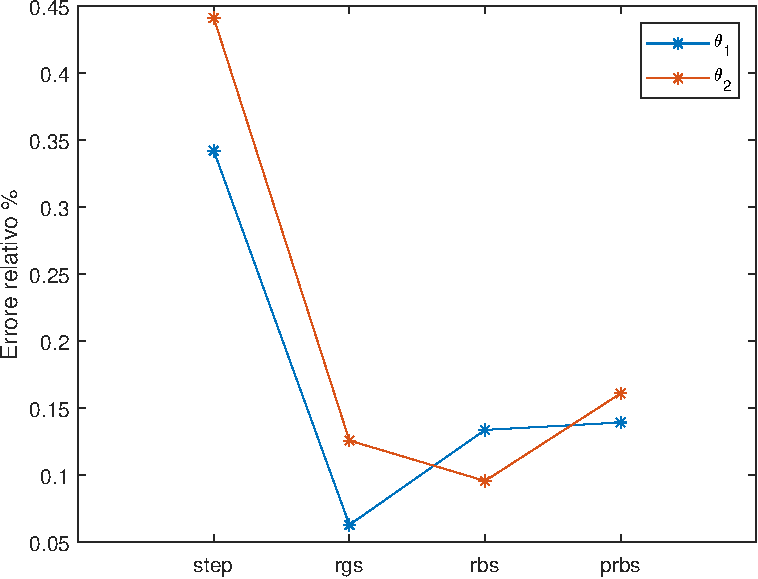
\includegraphics[width=0.95\linewidth]{error}
	\caption{Errore sui due parametri con i differenti segnali di ingresso utilizzati. Tra differenti ripetizioni dell'algoritmo l'errore potrebbe variare (sia a causa del metodo che della randomicità degli ingressi)}
\end{figure}
\section{Conclusioni}
\textcolor{blue}{\lipsum[1-2]}

%\pagebreak
\section*{Disponibilità dei dati}


\printbibliography[title=Riferimenti]
%\section*{References}
\pagebreak
\appendix
\section*{Appendice}
\lipsum[1-5]